\section{Risk-Based Stochastic Capital Budgeting using Conditional Value-at-Risk}
\label{sec:CVaR}

Value-at-Risk (VaR) is currently used by finance businesses to indicate the percentiles
of loss distributions. For instance, $95\%$-VaR is an upper estimate of losses which
is exceeded with $5\%$ probability. The popularity of VaR is mostly related to a simple
and easy to understand representation of high losses. However, VaR may have undesirable
mathematical characteristics such as a lack of subadditivity and convexity [Ref].
Another alternative percentile risk measure is called Conditional Value-at-Risk (CVaR),
which has more attractive properties than VaR, such as sub-additive and convex.
CVaR also called mean excess loss, mean shortfall, or tail VaR, is defined as the
expected loss exceeding VaR. In general, CVaR is the weighted average of VaR and
losses exceeding VaR. In this section, we will focus on using CVaR for capital
budgeting problem.

\subsection{Definitions of VaR and CVaR}
\label{definitionCVaR}
Let $X$ be a random variable with a cumulative distribution function
$F(z) = P{X\le z}$. It will be useful to think of $X$ as a ``loss'' or more generally
be such that large values are bad. The VaR of $X$ with confidence level
$\alpha$ (e.g., $\alpha = 0.9$ is:

\begin{equation}
VaR_\alpha (X) = \min {z|F_X(z)\ge \alpha}
\end{equation}

which is equivalent to $VaR_\alpha (X) = F_{X}^{-1}(\alpha)$ if $X$ is a continuous
random variable. By this definition, $VaR_\alpha (X)$ is a (lower) $\alpha$-percentile
of the random variable $X$. An alternative measure of risk is CVaR. Here, $CVaR_\alpha (X)$
is the conditional expectation of $X$ given that $X \ge VaR_\alpha (X)$.
Figure 28 shows the relationship between these two measures of risk.

\begin{figure}
    \centering
    \centerline{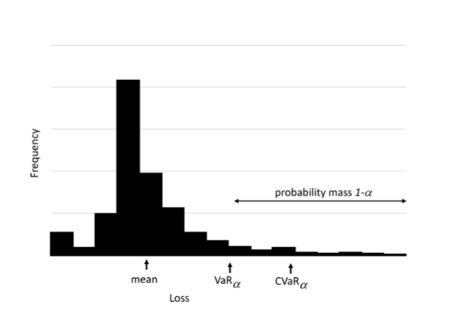
\includegraphics[scale=0.5]{CVaR.jpg}}
    \caption{Relationship between value-at-risk and conditional value-at-risk.}
    \label{fig:CVaR}
\end{figure}

The typical definition of $CVaR_\alpha (X)$ is $CVaR_\alpha (X) = E{X|X > VaR_\alpha (X)}$.
There are alternative ways to define this measure, which are mathematically equivalent.
Rockafellar and Uryasev in [Ref] (see also [Ref]) defines CVaR as:

\begin{equation}
CVaR_\alpha (X) = \min_\nu {\nu + 1/(1-\alpha) E[X-\nu]^+}
\end{equation}


\begin{equation}
f
\end{equation}

\begin{subequations}\label{WassersteinConstraints}
\begin{eqnarray}
f
\end{eqnarray}
\end{subequations}
